\documentclass[10pt,conference,onecolumn,compsoc]{IEEEtran}


\usepackage{hyperref}
\usepackage{enumitem}
\setlist[itemize]{leftmargin=3 cm}
\setlist[enumerate]{leftmargin=3cm}

% *** CITATION PACKAGES ***
\ifCLASSOPTIONcompsoc
  \usepackage[nocompress]{cite}
\else
  \usepackage{cite}
\fi

% *** GRAPHICS RELATED PACKAGES ***
\usepackage[pdftex]{graphicx}

% correct bad hyphenation here
\hyphenation{op-tical net-works semi-conduc-tor}


\begin{document}

\title{Leaping Llamas\\ for UTM CSCI 352 Spring 2017}

\author{Garrett Hay, Anderson Taylor, and Christina Hinton \\ % <-this % stops a space
}

\IEEEtitleabstractindextext{%
\begin{abstract}
We will be creating a similar game in the vein of Flappy Bird, which we are calling "Leaping Llamas." If the initial challenge proves to be trivial, we intend to add combat elements to increase the difficulty. Players looking for a casual yet challenging game should enjoy Leaping Llamas.
\end{abstract}
}
\maketitle

\IEEEdisplaynontitleabstractindextext
\IEEEpeerreviewmaketitle

\section{Introduction}
	The goal of this project is to create a simple yet fun game that can be played by anyone on a windows computer using only a mouse and keyboard.  For the type and content of the game we decided to go with a similar style to the popular game “Flappy Bird”.  At minimum we would like to include all of the basic functionality of the original game, so things like the auto generated level that is continuous and a high score system will definitely be incorporated into the app.
	
	Once all of the basic functionality described above is implemented we have plans to add additional functionality including variable difficulty settings and possibly even a “bullet hell” type game mode. We’re confident this will not only be an enjoyable experience for us the creators, but we also believe it will be fun for our peers to play post launch. By taking the “Flappy Bird” formula and making a more challenging experience, we think we can make a game that is relatively simple, but ultimately hard to master.
 

\subsection{Background}
	"Flappy Bird" is a game where the player controls a small bird, using inputs to lift the bird in order to navigate through pipes. Gravity pushes the bird down, but inputs can easily send the bird too high.

	If we reach our initial goals, we will convert Leaping Llamas into a bullet hell. A bullet hell is a game in which players must navigate through hordes of enemy projectiles without being hit. We believe it will make the game hilariously difficult and add an interesting twist to the Flappy Bird formula.

	We decided to tackle this project because it's a simple, universally-recognized game. It's known for being fun and addictive. We want to make a game that's cute, funny, and addicting, and a game like Flappy Bird is a fantastic inspiration to us.

\subsection{Challenges}
	We expect that insuring the player character's movement is smooth and responsive will be difficult. Hit boxes and fail states will be initially difficult. If we decide to have randomly generated pipes, we believe this will prove to be extremely tricky.

\section{Scope}
	Our main goal is to make Leaping Llamas, a simple Flappy Bird-like game. If we find ourselves finished well before the due date, we will add additional mechanics to further set it apart from Flappy Bird. Firstly, we would like to add bullet hell mechanics. Bullet hell mechanics are a usually extreme or hell-like amount of obstacles, usually bullet-like, that while challenging should be dodgable from somewhere on-screen.  Secondly, we would like to add onto the existing game in the form of animating objects, in order of: the background, the llama, any buttons, and any obstacles like 'pipes' and/or bullet-likes. 

\subsection{Requirements}
	As part of fleshing out the scope of your requirements, you'll also need to keep in mind both your functional and non-functional requirements.  These should be listed, and explained in detail as necessary.  Use this area to explain how you gathered these requirements.

\subsubsection{Functional}
	\begin{itemize}
	\item The game must be controlled with "Spacebar" key or "left-click" mouse button.
	\item The game must be implemented with C\# WPF.
	\item The game must feature music and sound effects.
	\item The game must feature obstacle generation with several different difficulty options.
	\item The game must be pausable with the "P" key.
	\end{itemize}

\subsubsection{Non-Functional}
	\begin{itemize}
	\item Security -- user credentials must be encrypted on disk, users should be able to reset their passwords if forgotten
	\item Performance -- Speed of obstacle generation.
	\item Scalability -- The obstacle generation will be potentially unlimited obstacle generation.
	\end{itemize}

\subsection{Use Cases}
	This subsection is arguably part of how you define your project scope (why it is in the Scope section...).  In a traditional Waterfall approach, as part of your requirements gathering phase (what does the product actually \emph{need} to do?), you will typically sit down with a user to develop use cases.

	You should have a table listing all use cases discussed in the document, the ID is just the order it is listed in, the name should be indicative of what should happen, the primary actor is typically most important in an application where you may have different levels of users (think admin vs normal user), complexity is a best-guess on your part as to how hard it should be.  A lower number in priority indicates that it needs to happen sooner rather than later.  A sample table, or Use Case Index can be seen in Table \ref{tab:useCaseIndex}.

\begin{table}
\centering
\begin{tabular}{|c|c|c|c|c|}
\hline
Use Case ID & Use Case Name & Primary Actor & Complexity & Priority \\
\hline \hline
1 & Start Window & User & Simple & 1\\
\hline
2 & Choose Difficulty & User & Simple & 1\\
\hline
3 & Playing \textit{Leaping Llamas} & User & Hard & 1\\
\hline
4 & Scoreboard after \textbf{Game Over} & System & Med & 1\\
\hline
5 & High Score Screen & System & Med & 1\\
\hline

\end{tabular}
\caption{Sample use case table}
\label{tab:useCaseIndex}
\end{table}

%Case 1
\begin{itemize}
\item[Use Case Number:] 1
\item[Use Case Name:] Start Window
\item[Description:] The user on the program starts the program. The user will choose whether to start the game, see the high scores, or exit the program.
\end{itemize}
\begin{enumerate}
\item The user shall press "Start" button.
\item The program go to the difficulty screen.
\item[Termination Outcome:] The user will go to Case: 2.
\end{enumerate}
Alternative: User chooses the "High Score" button
\begin{enumerate}
\item The user shall press "High Score" button.
\item The program go to the High Score screen.
\item[Termination Outcome:] The user will go to Case: 6.
\end{enumerate}
Alternative: User chooses the "Exit" button
\begin{enumerate}
\item The user shall press "Exit" button.
\item The program will end.
\item[Termination Outcome:] The user has kill the program.
\end{enumerate}


%Case 2
\begin{itemize}
\item[Use Case Number:] 2
\item[Use Case Name:] Choose difficulty
\item[Description:] The user on the program chooses what difficulty for the game. The user will be shown the controls for the game.
\end{itemize}

\begin{enumerate}
\item The user shall press "Easy" button.
\item The screen shall show the controls for the proceeding game.
\item[Termination Outcome:] The user has chosen the difficulty and will be sent to the game.
\end{enumerate}

Alternative: User chooses Medium difficulty
\begin{enumerate}
\item The user shall press "Medium" button.
\item The screen shall show the controls for the proceeding game.
\item[Termination Outcome:] The user has chosen the difficulty and will be sent to the game.
\end{enumerate}

Alternative: User chooses Hard difficulty
\begin{enumerate}
\item The user shall press "Hard" button.
\item The screen shall show the controls for the proceeding game.
\item[Termination Outcome:] The user has chosen the difficulty and will be sent to the game.
\end{enumerate}

Alternative: User chooses "Back" button
\begin{enumerate}
\item The user shall press "Back" button.
\item The program shall return to the Starting screen.
\item[Termination Outcome:] The user has chosen to go back to the Case: 1 screen.
\end{enumerate}


%Case 3
\begin{itemize}
\item[Use Case Number:] 3
\item[Use Case Name:] Playing \textit{Leaping Llamas}
\item[Description:] The user on the program starts the game. The user will make the llama leap over and between the obstacles until the llama hits a obstacle. This will send the user to the scoreboard.
\end{itemize}

\begin{enumerate}
\item The user shall press "Spacebar" button to "Leap" over obstacles.
\item The game will count up by 1 for each obstacle on its counter.
\item The game will end once the user's Llama hits an obstacle
\item[Termination Outcome:] The user has played the game portion of the program.
\end{enumerate}


%Case 4
\begin{itemize}
\item[Use Case Number:] 4
\item[Use Case Name:] Scoreboard after 'Game Over'
\item[Description:] A shopper on our site has finished shopping.  They will click on a ``Checkout" button.  This will kick off a process to calculate cart total, any taxes, shipping rates, and collect payment from the shopper.

\end{itemize}

\begin{enumerate}
\item The program shall open a window with the user's score and a "Retry" and "Next" buttons.
\item The user shall select "Retry" button and proceed back to Use Case: 1 until selecting the "Next" button.
\item[Termination Outcome:] The user will either replay the game with new score or proceed to the High Score screen.
\end{enumerate}

Alternative: The user scored a High Score
\begin{enumerate}
\item The program shall open a window with a text box and shall prompt the user for a username and a "Retry" and "Next" buttons.
\item The username shall be stored along with the user's score to a file with other High scores.
\item The user shall select "Retry" button and proceed back to Use Case: 1 until selecting the "Next" button.
\item[Termination Outcome:] The user will either replay the game with new score or proceed to the High Score screen.
\end{enumerate}


%Case 5
\begin{itemize}
\item[Use Case Number:] 5
\item[Use Case Name:] High Score screen
\item[Description:] A user has finished playing. The user will be shown the top 10 High Scores on the game. They will choose either to play again or return to the title screen.

\end{itemize}

\begin{enumerate}
\item The window shall display the High scores in nonincreasing order from the top of the window.
\item The user shall choose whether to click the "Retry" button.
\item The program will return to the game on the same difficulty.
\item[Termination Outcome:] The user will either replay the game with new score.
\end{enumerate}

Alternative: The user chooses the "Title" button
\begin{enumerate}
\item The window shall display the High scores in nonincreasing order from the top of the window.
\item The user shall choose whether to click the "Title" button.
\item The program will return to the title screen.
\item[Termination Outcome:] The user will be at the Title screen at case: 1. 
\end{enumerate}

\begin{figure}[ht!]
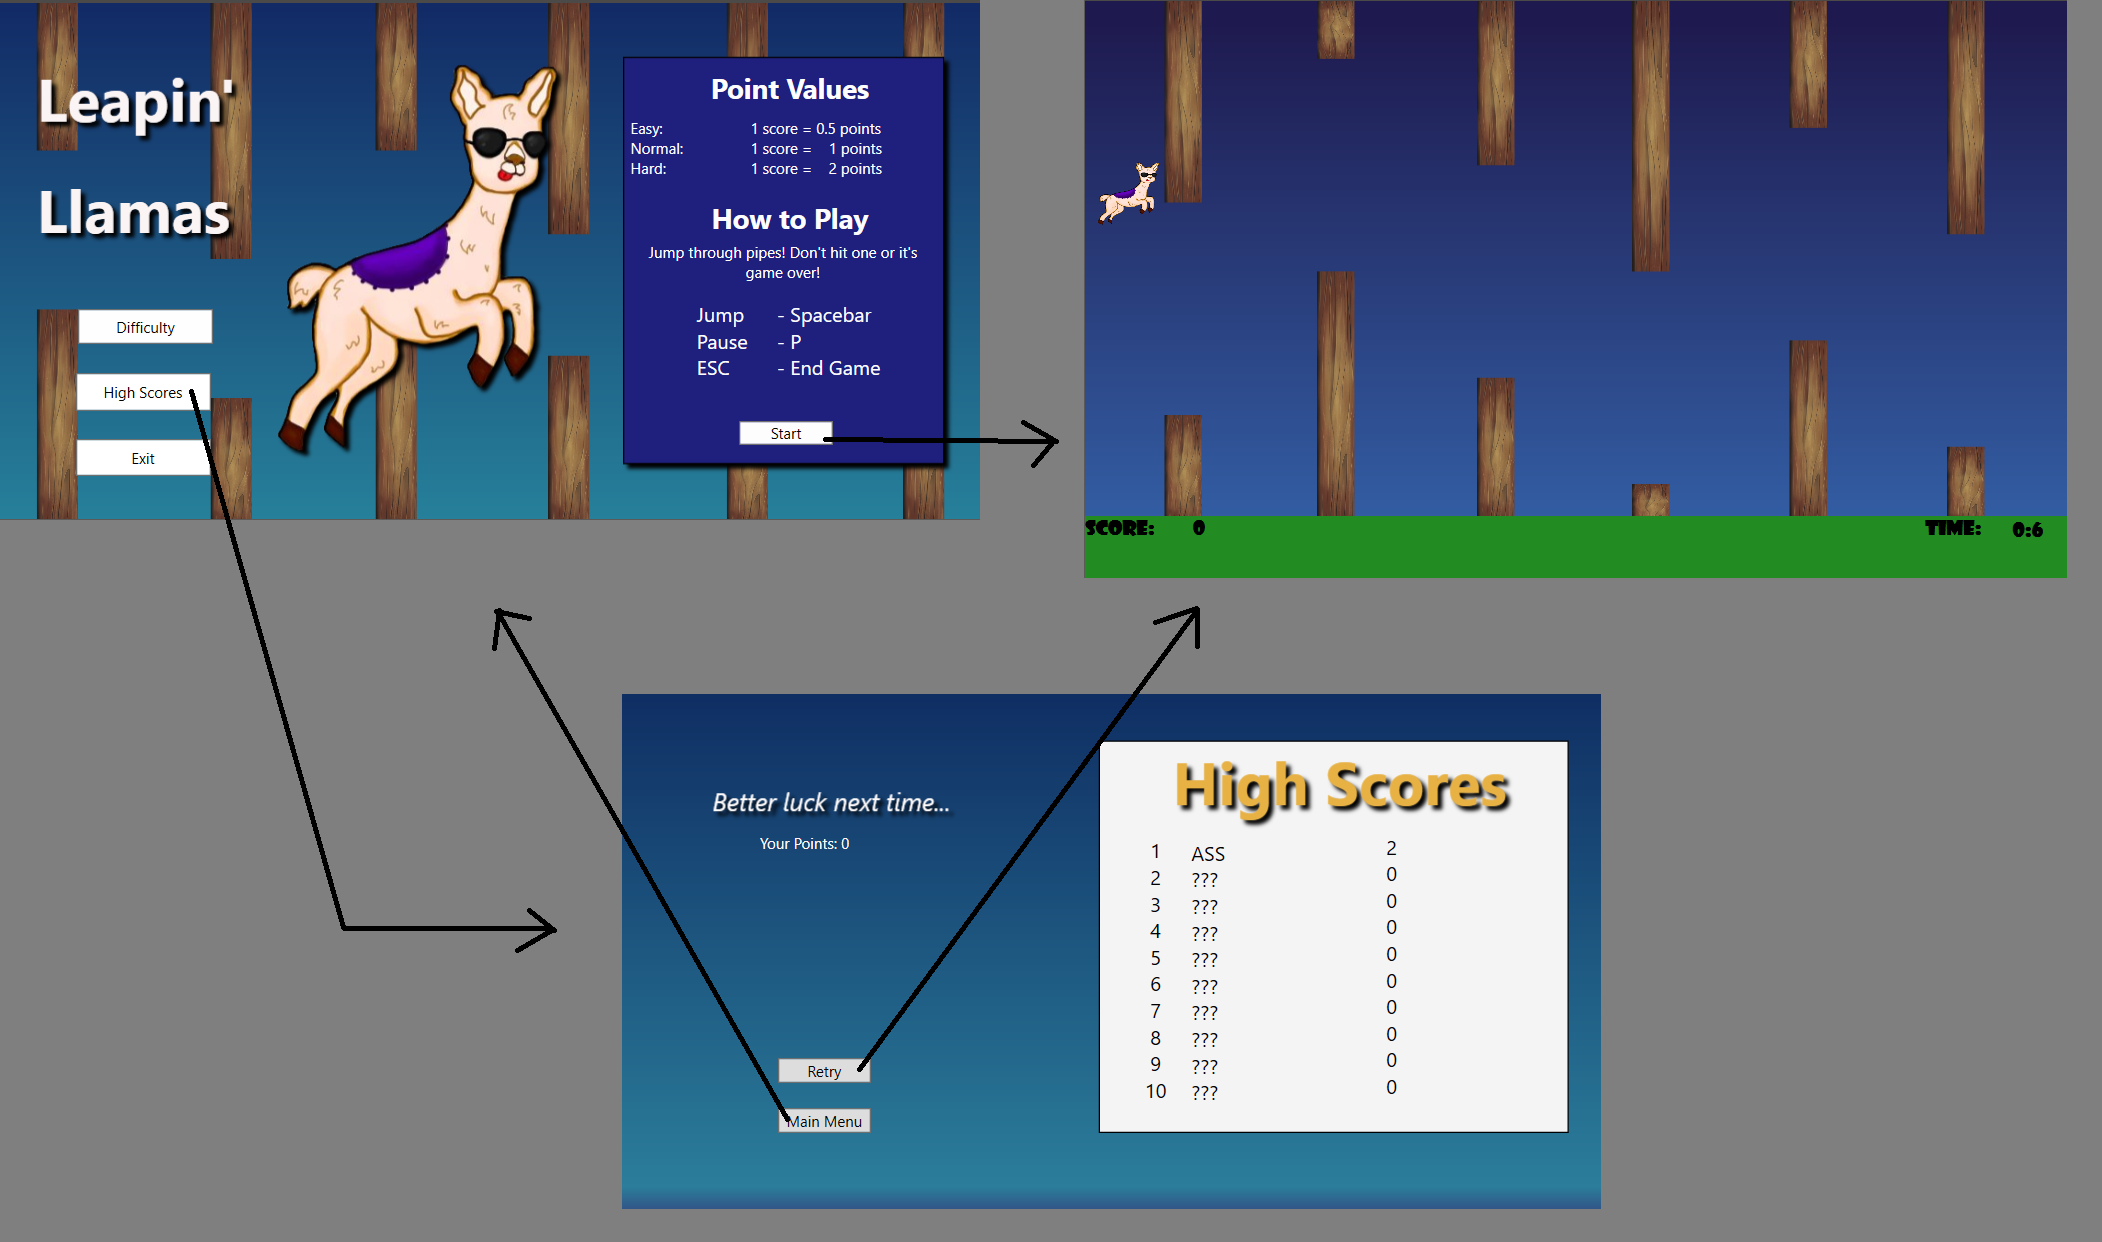
\includegraphics[height=250px, width=350px]{Mockup.png}
\caption{First picture, This is full number of Mock-Interfaces planned.}
\label{fig:mockup}
\end{figure}



\subsection{Interface Mockups}
For all below see Figure \ref{fig:mockup}
First in order, the user will begin on the 'Title' screen and choose one of the button to move to the corresponding screen. Next the 'Difficulty' screen buttons will all lead to the 'Game' screen. The 'Game' screen will always lead to the 'Score' screen at the end of the game. The 'Score' screen has two choices as follows. Lastly, the 'Highscore' screen will lead to two different options as follows.

\section{Project Timeline}
See Figure \ref{fig:timeline} below.
\begin{figure}[ht!]
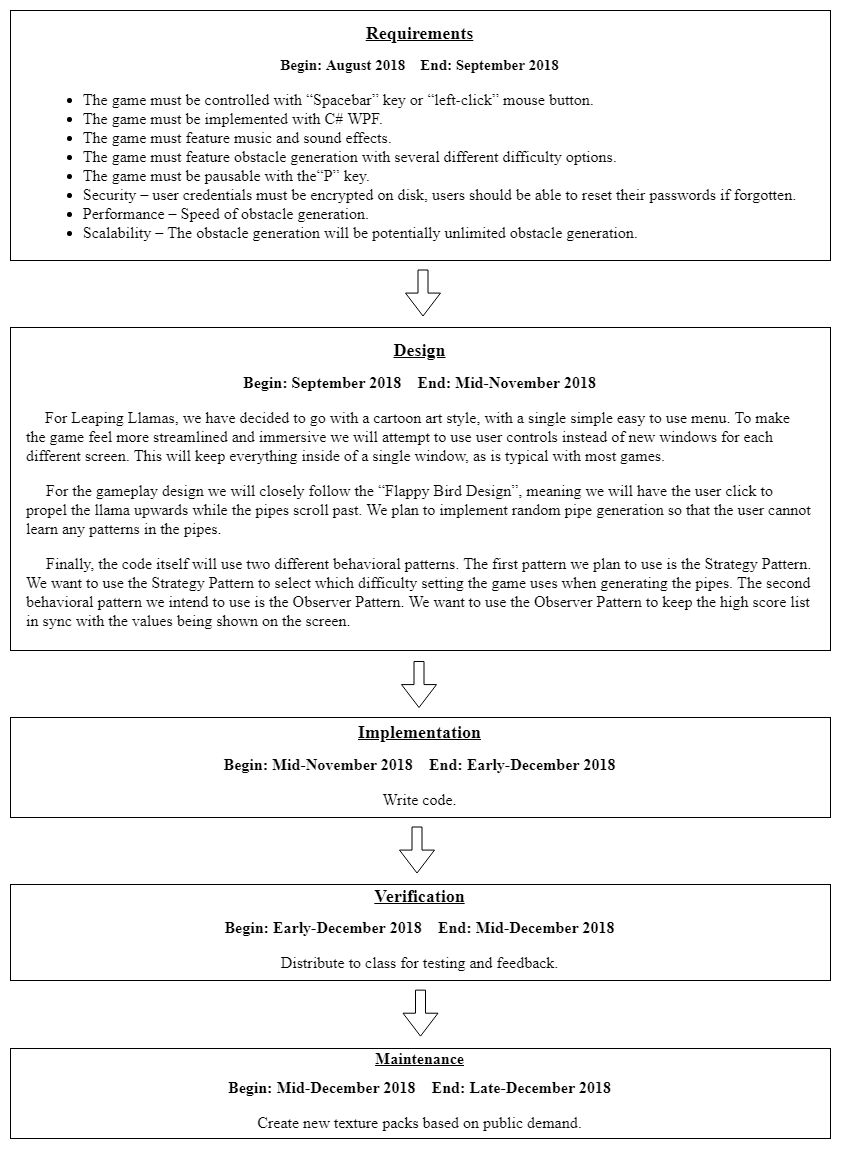
\includegraphics[height=600px, width=450px]{ProposalTimeline.png}
\caption{Proposed timeline, This is a rough estimate of the project timeline.}
\label{fig:timeline}
\end{figure}

\section{Project Structure}
At first, this will be a little empty (it will need to be filled in by the time you turn in your final report).  This is your chance to discuss all of your design decisions (consider this the README's big brother).

\subsection{UML Outline}
Show the full structure of your program.  Make sure to keep on updating this section as your project evolves (you often start out with one plan, but end up modifying things as you move along).  As a note, while Dia fails miserably at generating pdfs (probably my fault), I have had much success with png files.  Make sure to wrap your images in a \texttt{figure} environment, and to reference with the \texttt{ref} command.  For example, see Figure \ref{cat2}.

%\begin{figure}[ht!]
%\includegraphics[scale=1.5]{cat2.jpg}
%\caption{Your figures should be in the \emph{figure} environment, and have captions.  Should also be of diagrams pertaining to your project, not random internet kittens}
%\label{cat2}
%\end{figure}


\subsection{Design Patterns Used}
Make sure to actually use at least 2 design patterns from this class.  This is not normally part of such documentation, but largely just specific to this class -- I want to see you use the patterns!


\section{Results}
This section will start out a little vague, but it should grow as your project evolves.  With each deliverable you hand in, give me a final summary of where your project stands.  By the end, this should be a reflective section discussing how many of your original goals you managed to attain/how many desired use cases you implemented/how many extra features you added.

\subsection{Future Work}
Where are you going next with your project?
For early deliverables, what are your next steps?  (HINT: you will typically want to look back at your timeline and evaluate: did you meet your expected goals?  Are you ahead of schedule?  Did you decide to shift gears and implement a new feature?)
By the end, what do you plan on doing with this project?  Will you try to sell it?  Set it on fire?  Link to it on your resume and forget it exists?

\begin{thebibliography}{1}

\bibitem{IEEEhowto:kopka}
H.~Kopka and P.~W. Daly, \emph{A Guide to \LaTeX}, 3rd~ed.\hskip 1em plus
  0.5em minus 0.4em\relax Harlow, England: Addison-Wesley, 1999.

\end{thebibliography}

\begin{IEEEbiography}{Michael Shell}
Biography text here.
\end{IEEEbiography}

\begin{IEEEbiographynophoto}{John Doe}
Biography text here.
\end{IEEEbiographynophoto}

\begin{IEEEbiographynophoto}{Jane Doe}
Biography text here.
\end{IEEEbiographynophoto}
\end{document}


